\documentclass[fontset=none]{ctexbeamer}
% \documentclass[aspectratio=169]{ctexbeamer}

\usepackage{graphicx,array,caption,listings,fontawesome,bookmark}

\makeatletter

\@namedef{ver@beamerfontthememetropolis.sty}{9999/99/99}

% Beamer theme
\usetheme{Xiaoshan}
\usefonttheme{serif}

% Beamer settings
\metroset{sectionpage=simple}
\setbeamerfont{title}{size=\huge, series=\bfseries}
\setbeamerfont*{subtitle}{size=\large, shape=\itshape}
\setbeamerfont{section title}{size=\Large, series=\bfseries}
\setbeamerfont{frametitle}{size=\large, series=\bfseries}
\setbeamerfont{caption}{size=\footnotesize, series=\bfseries}
\setbeamerfont{footnote}{size=\tiny}
\setbeamerfont{alerted text}{series=\bfseries}
\addtobeamertemplate{institute}{\raggedleft}{}
\setbeamertemplate{title}{%
  \raggedleft
  \linespread{1.0}%
  \inserttitle
  \hspace*{1.2cm}\par
  \vspace*{0.5em}}
\setbeamertemplate{subtitle}{%
  \raggedleft
  \insertsubtitle
  \hspace*{1.2cm}\par
  \vspace*{0.5em}}
\setbeamertemplate{frame numbering}{\zhdigits[style=Financial]{\insertframenumber}}

% CTeX settings
\ctexset{punct=kaiming}

% Colors
\colorlet{keyword}{松花绿}
\colorlet{comment}{漆黑!50}
\colorlet{texcs}{酡红}
\colorlet{emph}{靛蓝}

% Fonts
\setmainfont{Libertinus Serif}[Scale=1.1, BoldFont=* Bold]
\setmonofont{Iosevka}
\setCJKmainfont{Source Han Serif SC}[%
  UprightFont=* SemiBold, BoldFont=* Heavy, ItalicFont=* SemiBold, RawFeature=+fwid]
\setCJKmonofont{Sarasa Mono SC}

% Graphics
\captionsetup[figure]{labelformat=empty, justification=centering}

% PDF bookmark
\apptocmd{\beamer@@frametitle}{%
  \only<1>{\expandafter\ifnum\insertcontinuationcount<2\relax
    \bookmark[page=\the\c@page,level=4]{#1}\fi}}{}{}

% Code listings
\lstdefinestyle{style@latex}{
  language        = [latex]TeX,
  alsoletter      = {*},
  basewidth       = 0.54em,
  escapeinside    = {(*}{*)},
  basicstyle      = \small\ttfamily,
  keywordstyle    = \bfseries\color{keyword},
  commentstyle    = \itshape\color{comment},
  texcsstyle      = *\color{texcs},
  emphstyle       = \itshape\color{emph},
  numbersep       = 4pt,
}
\lstnewenvironment{texcode}[1][]{\lstset{%
  style=style@latex,
  gobble=2,
  morekeywords={\documentclass,\usepackage,\begin,\end},#1}}{}

% Hack
% Use small caps for LaTeX symbol
\DeclareRobustCommand{\LaTeX}{%
  L\kern-.3em%
  \raisebox{.2em}{\textsc{a}}\kern-.14em%
  \TeX}
% PoZheHao, see https://github.com/CTeX-org/ctex-kit/issues/382
\ExplSyntaxOn
\xeCJK_new_class:n { PoZheHao }
\__xeCJK_save_CJK_class:n { PoZheHao }
\xeCJK_declare_char_class:nn { PoZheHao } { "2014 }
\seq_map_inline:Nn \g__xeCJK_class_seq
  {
    \str_if_eq:nnF {#1} { PoZheHao }
      {
        \xeCJK_copy_inter_class_toks:nnnn { PoZheHao } {#1} { FullRight } {#1}
        \xeCJK_copy_inter_class_toks:nnnn {#1} { PoZheHao } {#1} { FullRight }
      }
  }
\ExplSyntaxOff

% Macros
\newcommand\enparen[1]{(\raisebox{0.2ex}{#1})}
\newcommand\link[1]{\href{#1}{\faLink}}

% Information
\title{现代 \LaTeX{} 入门讲座}
\subtitle{Introduction to Modern \LaTeX{}}
\author{曾祥东}
\institute{复旦大学\quad 物理系}
\date{\zhdate{2018/12/6}}

\makeatother

\begin{document}

\maketitle

\section{介绍}

\begin{frame}{历史回眸}
\begin{columns}
\begin{column}{0.45\textwidth}
  \begin{figure}
    \centering
    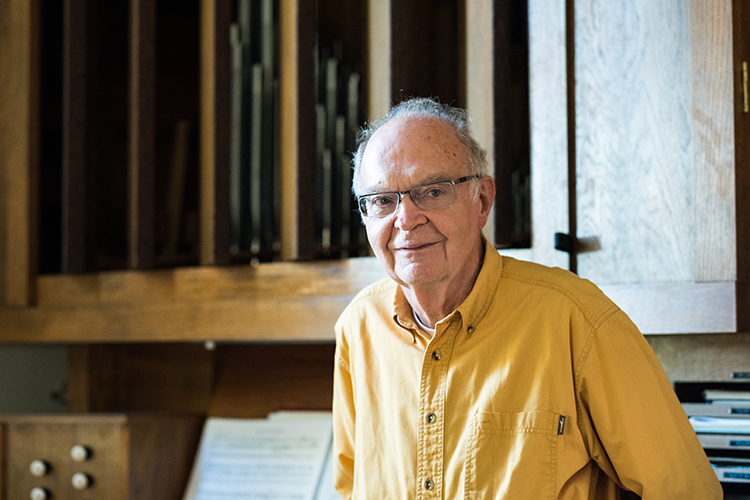
\includegraphics[height=3.2cm]{figures/Knuth-vivian20181019E.jpg}
    \caption{高德纳(Donald~E. Knuth)\footnotemark \\ \TeX}
  \end{figure}
\end{column}
\begin{column}{0.45\textwidth}
  \begin{figure}
    \centering
    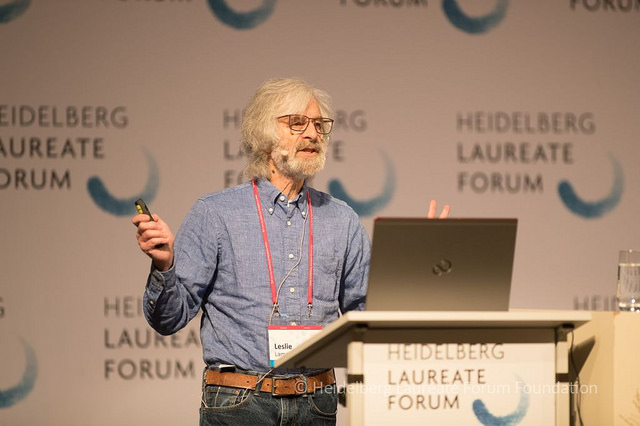
\includegraphics[height=3.2cm]{figures/lamport-2018.jpg}
    \caption{Leslie Lamport~\footnotemark \\ \LaTeX}
  \end{figure}
\end{column}
\end{columns}
\footnotetext[1]{图片来源:~\url{https://www-cs-faculty.stanford.edu/~knuth/graphics.html}}
\footnotetext[2]{图片来源:~\url{https://aperiodical.com/2018/09/hlf-blogs-leslie-lamport-thinks-your-code-is-bad}}
\end{frame}

\begin{frame}{\LaTeX{} 是什么?}
\begin{itemize}
  \item 打公式方便?
  \item 写论文神器?
  \item 排版语言 + 标记语言 + 宏语言?
\end{itemize}
\end{frame}

\begin{frame}[fragile]
\frametitle{\LaTeX{} 是什么?\mbox{}——\mbox{}“What you think is what you get!”}
\begin{columns}
\begin{column}{0.48\textwidth}
  \begin{texcode}[basicstyle=\tiny\ttfamily, moretexcs={\maketitle},
    emph={equation,itemize,document}]
  \documentclass{article}
  \usepackage{amsmath,graphicx}
  \title{Normal distribution}
  \author{Wikipedia, the free encyclopedia}

  \begin{document}
  \maketitle
  \section{Introduction}
  % 省略一些内容……
  The probability density of the normal
  distribution is
  \begin{equation}
    f(x|\mu, \sigma)
    = \frac{1}{\sqrt{2\pi\sigma^2}}
      e^{-\frac{(x-\mu)^2}{2\sigma^2}}
  \end{equation}
  where
  \begin{itemize}
    \item $\mu$ is the mean of the distribution
    \item $\sigma$ is the standard deviation
  \end{itemize}
  \end{document}
  \end{texcode}
\end{column}
\begin{column}{0.48\textwidth}
  \begin{figure}
    \centering
    \vspace{-0.8cm}
    \includegraphics[width=\textwidth]{normal-dist/normal-dist.pdf}
  \end{figure}
\end{column}
\end{columns}
\end{frame}

\begin{frame}{基本原则}
\begin{itemize}
  \item 排版 \textit{vs} 文字处理
    \begin{itemize}
      \item 《别把 \LaTeX{} 当 Word 用》
    \end{itemize}
  \item 遵循业\enparen{xué}界\enparen{xiào}规范
    \begin{itemize}
      \item 《管教务处 \textit{or} 研究生院 \textit{or} 物理系叫爸爸》
    \end{itemize}
  \item 追求良好的阅读体验\enparen{readability}
  \item 内容与格式分离
  \item \alert{内容永远比格式重要!}
\end{itemize}
\end{frame}

\section{安装}

\begin{frame}{选择发行版}
\begin{itemize}
  \item \TeX{} 发行版\enparen{distribution}
    \begin{itemize}
      \item 引擎、宏包、字体、文档的综合体
      \item 类比 Visual Studio
      \item \TeX{} Live、Mac\TeX{}、W32\TeX{}、MiK\TeX{} 等
    \end{itemize}
  \item \TeX{} Live \link{https://www.tug.org/texlive}
    \begin{itemize}
      \item 官方维护,首选,跨平台
      \item Mac\TeX{} ≈ macOS 下的 \TeX{} Live
      \item 缺点:体积大\enparen{3GB+}、每年需要重装
    \end{itemize}
  \item MiK\TeX{} \link{https://miktex.org}
    \begin{itemize}
      \item 由 Christian Schenk 维护(是个狠人)
      \item 宏包随用随装
      \item 缺点:曾经只有 Windows 版本、网络问题
    \end{itemize}
  \item \alert{不要安装 \CTeX{} 套装!}
    \begin{itemize}
      \item \alert{存在严重 bug,并且完全过时}
    \end{itemize}
\end{itemize}
\end{frame}

\begin{frame}{下载}
\begin{itemize}
  \item 选择国内 CTAN 镜像
    \begin{itemize}
      \item 清华大学开源软件镜像站 \link{https://mirrors.tuna.tsinghua.edu.cn}
      \item 上海交通大学软件源镜像服务 \link{https://mirrors.sjtug.sjtu.edu.cn}
      \item 中国科学技术大学开源软件镜像 \link{https://mirrors.ustc.edu.cn}
      \item 复旦大学……不存在的
    \end{itemize}
  \item 建议使用 ISO 安装
  \item 在线安装要求网络稳定
\end{itemize}
\end{frame}

\begin{frame}{安装流程}
\begin{itemize}
  \item 新手建议安装完整版 \TeX{} Live 或 Mac\TeX{}
    \begin{itemize}
      \item 一路点击“下一步”
      \item 保持耐心,做好重装的打算
    \end{itemize}
  \item Linux specials
    \begin{itemize}
      \item 软件源更新较慢,推荐 Vanilla \TeX{} Live
      \item 环境变量、\texttt{fontconfig} 配置
    \end{itemize}
\end{itemize}
\end{frame}

\begin{frame}{神圣的战争——选择编辑器}
  
\end{frame}

\iffalse

\section{填写内容}
\section{改变样式}

\fi
\end{document}
